\documentclass[10pt]{beamer}
\usepackage[utf8]{inputenc}
\usetheme{Berlin}
\usecolortheme{whale}
\usepackage{tikz}
\usetikzlibrary{automata,positioning}
\usepackage{booktabs}
\usepackage{chronology}
\usepackage{graphicx}
\graphicspath{ {./} }
\usetikzlibrary{arrows}
\definecolor{myGreen}{RGB}{0, 107, 61}
\definecolor{myGreen2}{RGB}{151, 199, 163}
\definecolor{myCyan}{RGB}{128, 179, 153}

\setbeamercolor{footnote mark}{fg=white}
\makeatletter
\makeatother
\setbeamertemplate{section in toc}{\hspace\inserttocsection}
\title{\textbf{Student Companion | Initial Presentation}}
\author{\textbf{Chaotic Programmers}     \\213050082: Gautam Bhavana\\
21q050004: Abisek R K\\
213050027: Sakharam Sahadeo Gawade\\}
\institute{IIT Bombay}
\date{September 29, 2021}

\begin{document}
{\maketitle}
\section[]{}
\begin{frame}{Topics to cover}
\tableofcontents
\end{frame}
\section{Introduction and Motivation}
\begin{frame}{Introduction and Motivation}
    \begin{block}{\large Introduction}
{\textit{Online semester made us realize the importance of group studies. Also, students who do distance learning or take any online course find it difficult to keep phase with the course and leaves little time for revision. We propose a website which will keep students motivated by checking their phase with friends and do timely revision.}}
\end{block}
\pause
\begin{block}{\large Motivation}
{\textit{Flash cards are used  as a self-testing technique and the efficacy is determined by the amount and timings of practice. \cite{flashcard} \\The pandemic has affected academic delivery and collaborative learning. A tool for revision and sharing flashcards can enhance the learning process and a leaderboard provides a virtual competitive environment and enhances learner's motivation.\cite{leaderboard}}}
\end{block}
\end{frame}
\begin{frame}{Introduction and Motivation}
   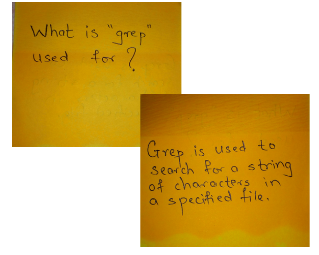
\includegraphics[scale=0.385]{Flashcard.png}
   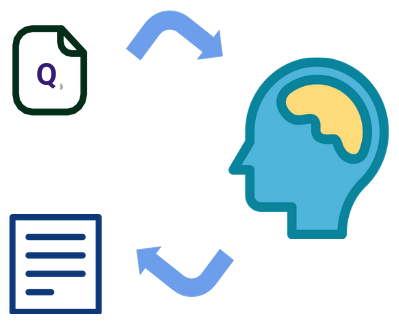
\includegraphics[scale=0.292]{Active_recall.png}
   \centering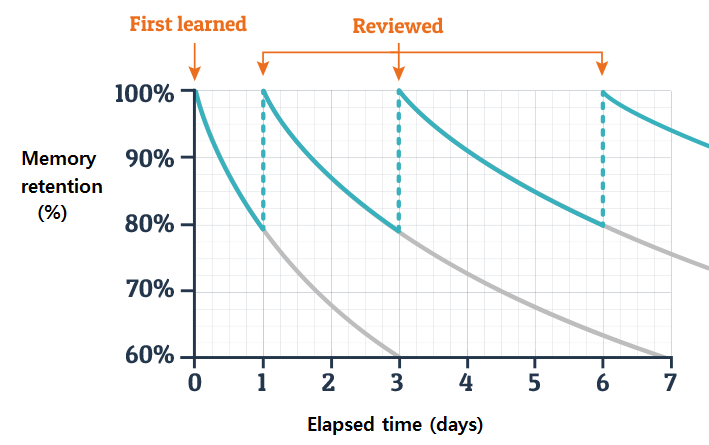
\includegraphics[scale=0.22]{forgetting_curve.png}\tiny{\cite{forgetting-curve}}
\end{frame}
\section{Problem Statement}
\begin{frame}{Problem Statement}
Building a website to create a study tool which uses flashcards and timed revisions for learners and help them cope up with online education by providing a competitive feel with their friends along with sharing their flashcards to give them feel of a virtual group study environment.\\

\end{frame}
\section{Methodology}
\begin{frame}{Methodology}
\begin{itemize}
    \item Use of Flash cards to help capture points to remember.
    \item Revision of flashcards, facilitating "Active Recall".
    \item Timely repeated revisions using "Spaced Repetition" strategy to retain information in memory longer.
    \item Allow users to share Flash cards with friends, creating a virtual "Group Study" like environment.
    \item Provide leader boards to encourage friendly competitions among students.
\end{itemize}

\end{frame}
\section{Technologies Used}

\begin{frame}{Technologies Used}
\begin{enumerate}
    \item Django - Framework to be used for Backend.
    \item AngularJS - For making responsive GUI.
    \item MySQL - For storing data.
    \item Github - For Version Control
    \item \LaTeX - For Presentation
    \item Sphinx - For Documentation

\end{enumerate}

\begin{figure}
    \centering
    
\includegraphics[scale=0.3]{Tech.png}
    \caption{Web Technologies \cite{Django}\cite{AngularJS}\cite{MySQL}}
    \label{fig:3tech}
\end{figure}

\end{frame}
\section{Timeline}
\begin{frame}{Timeline}
\begin{chronology}[2]{0}{27}{\textwidth}
\event[0]{2}{Learning Technologies}
\event[3]{9}{Skeleton of website}
\event[10]{16}{Code the Modules}
\event[17]{25}{Touch-up, Testing}
\event{27}{Project PPT}
\end{chronology}
\begin{center}
\begin{tabular}{ |c|c|  } 
 \hline
 Oct 3 & Learning Technologies\\
 &\\
 \hline
 Oct 10 &  A skeleton of the project (front end+backend+database design) \\ 
 &\\
 \hline
  Oct 17 & CRUD Flashcards [Bhavana]\\
   & Scheduling and Leaderboard [Sakharam]\\
   & Sharing and Friends [Abisek]\\
 \hline
  Oct 25 & Touch-ups, Testing\\
  \hline
\end{tabular}
\end{center}
\end{frame}
\section{Testing Criteria}
\begin{frame}{Testing Criteria}
    \begin{itemize}
        \item The Site should run on local servers and should be compatible across modern browsers.
        \item Creating, Editing and Deletion of Flashcards should be seamless.
        \item Users must have a login facility.
        \item Users should have the ability to share Flashcards with their friends by specifying their email.
        \item Users must be able to compare their progress against the leader board.
        \item Users must have automated, dynamic revision of flashcards scheduled to them, based on past performance.
    \end{itemize}
\end{frame}
\section{Deliverables}
\begin{frame}{Deliverables}
\begin{enumerate}
    \item Login page for user to login
    \item Facility to create, edit and delete flashcards
    \item Spaced Repetition of flashcards
    \item Adding friends and sharing cards among friends
    \item A leaderboard among friends
    \item Decks to organize cards
    \item Creating a custom decks from existing cards for custom revision
    \item An internal timer to keep cards in front next time during revision if recalling too longer
    \item Show current progress of cards for the user and user's friends
\end{enumerate}
\end{frame}
\section{References}
\begin{frame}
        \frametitle{References}
        \footnotesize\bibliographystyle{amsalpha}
        \bibliography{./references.bib}
\end{frame}
\end{document}